\documentclass[a4page, 11pt, showtrims]{memoir}
\semiisopage

\chapterstyle{veelo}
%% KAPITULU FORMATU BATZUK ARAZOAK EMATEN DITUZTE DOKUMENTUA 
%% MOZTERAKOAN (croppedsize AUKERAREKIN, BEHEAN AGERTZEN DENA). 
%% JARRAIAN ALTERNATIBA SGURU BATZUK DAUDE

%\chapterstyle{default}
%\chapterstyle{bianchi}
%\chapterstyle{brotherton}
%\chapterstyle{demo2}
%\chapterstyle{ell}
%\chapterstyle{ger}
%\chapterstyle{wilsondob}


\pdfobjcompresslevel 0



%% PAKETE HONEN AGINDUAK ERABILTZEN BADIRA, ALDATU HIZKUNTZA AUKERA %%
%% SI SE USAN LOS COMANDOS DE ESTE PAQUETE, CAMBIAR LA OPCIÓN DE IDIOMA %%
\usepackage[es]{ifcommands}


%% INFORMAZIOA / INFORMACIÓN %%
\newcommand{\egilea}{Martín López de Ipiña Muñoz}
\newcommand{\zuzendariak}{
  Galdos Otermin, Aritz \\
  Pereira Varela, Juanan \\
  Azanza Sesé, Maider
}
\newcommand{\izenburua}{Título del trabajo}
\newcommand{\data}{\today}


%% BAKARRIK BAT DESKOMENTATU, GRADU AMAIERAKO LANA BADA. BESTELA, DENAK KOMENTATU%%
%% DESCOMENTAR SOLO UNO SI ES UN TRABAJO FIN DE GRADO. SINO, COMENTAR TODOS%%

%\newcommand{\ikasketak}{Informatika Ingeniaritzako Gradua}
\newcommand{\ikasketak}{Grado en Ingeniería Informática}
%\newcommand{\ikasketak}{Adimen Artifizialeko Gradua}
%\newcommand{\ikasketak}{Grado en Inteligencia Artificial}


%% BAKARRIK BAT DESKOMENTATU, INGENIARITZA INFORMATIKAKOA BADA. BESTELA, DENAK KOMENTATU %%
%% DESCOMENTAR SOLO UNO SI ES EN INGENIERÍA INFORMÁTICA. SINO, COMENTAR TODOS %%

%\newcommand{\espezialitatea}{Konputazioa}
%\newcommand{\espezialitatea}{Computación}
%\newcommand{\espezialitatea}{Software Ingeniaritza}
\newcommand{\espezialitatea}{Ingeniería de Software}
%\newcommand{\espezialitatea}{Konputagailuen Ingeniaritza}
%\newcommand{\espezialitatea}{Ingeniería de Computadores}


%% BAKARRIK BAT DESKOMENTATU MASTER AMAIERAKO LANA BADA. BESTELA, DENAK KOMENTATU%%
%% DESCOMENTAR SOLO UNO SI ES UN TRABAJO FIN DE MASTER. SINO, COMENTAR TODOS%%

%\newcommand{\ikasketak}{Máster Universitario en Ingeniería Computacional y Sistemas Inteligentes}
%\newcommand{\ikasketak}{Konputazio Ingeniaritza eta Sistema Adimentsuak Unibertsitate Masterra}

%% TESIENTZAKO KONFIGURATU
%\newcommand{\saila}{Department of Computer Science and Artificial Intelligence}
%\newcommand{\phdarloa}{Computer Science}
%% KOMENTATU A4 FORMATUAN ATERATZEKO, FORMATU TXIKIAGOAN AGERTZEKO 
%% GERO INPRIMATZEKO. MOZTEKO MARKAK IKUSTEKO GEHITU showtrims AUKERA
%% memoir KLASEAREN ARGUMENTUETAN
%\newcommand{\croppedsize}

%% DOKUMENTUAREN HIZKUNTZA / IDIOMA DEL DOCUMENTO %%
%% BAKARRIK BAT DESKOMENTATU / DESCOMENTAR SOLO UNO %%
%\newcommand{\euskaraz}
\newcommand{\castellano}
%\newcommand{\english}


\input config/macros

\title{\izenburua}
\author{\egilea}
\date{\data}


\begin{document}

%% AZALA BEREZIRIK BADUZU (PDF FORMATUAN), DESKOMENTATU%%
%% SI HAY UNA PORTADA ESPECIAL (EN PDF), DESCOMENTAR%%
	
%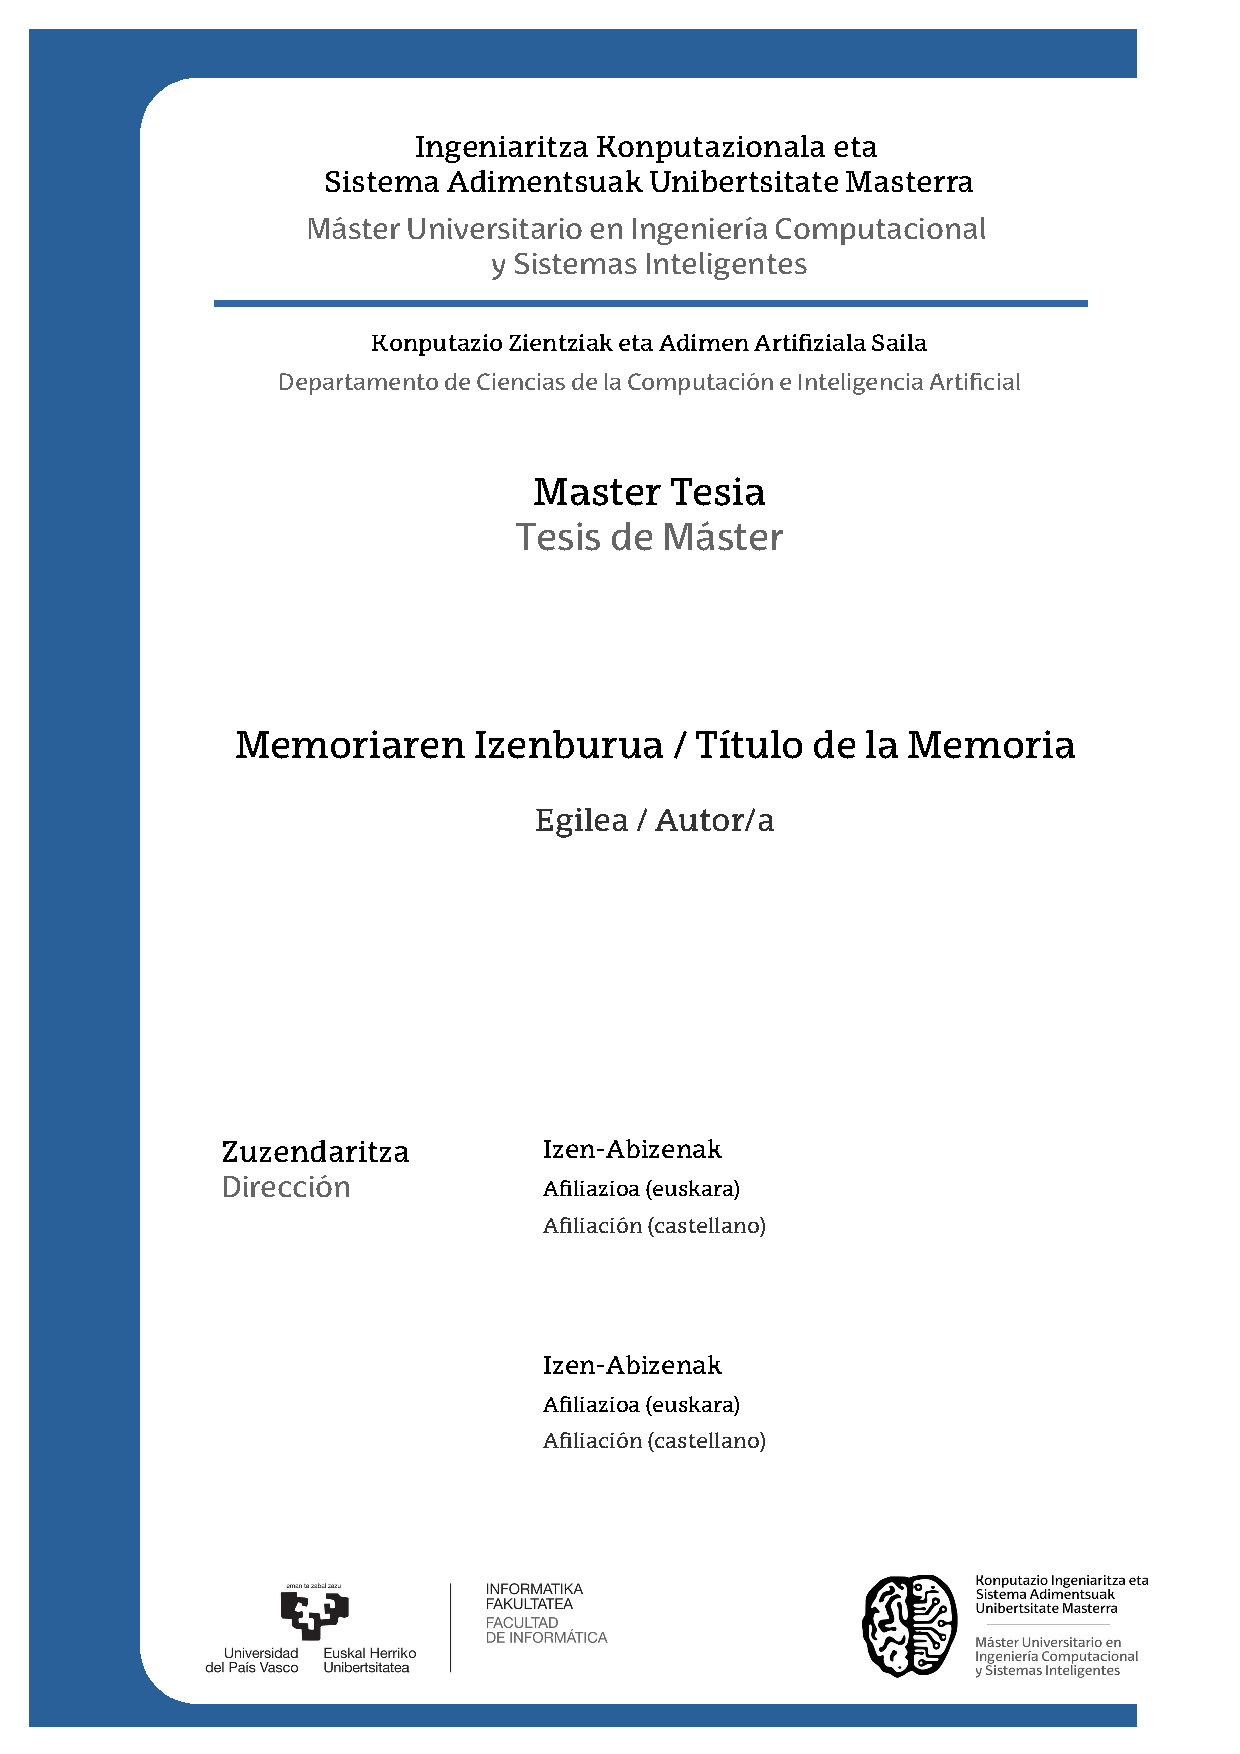
\includepdf[pages={1-}]{cover.pdf}
%\cleardoublepage


%% AUKERATU DAGOKIONA. AZALA BEREZIA GEHITUZ GERO, KOMENTATU DAITEKE, BETIERE HEMENGOAN AGERTZEN DEN INFORMAZIOA AGERTZEN BADA %%
%% SELECCIONA LA QUE CORRESPONDA. EN CASO DE TENER UNA PORTADA ESPECIAL SE PUEDE COMENTAR, SIEMPRE Y CUANDO DICHA PORTADA INCLUYA LA INFORMACIÓN QUE APARECE EN ESTA%%

\input config/cover_informatika
%\input config/cover_adimen_artifiziala
%\input config/cover_masterra
%\input config/cover_phd_dissertation

\cleardoublepage
\frontmatter

%%%%%%%%%%%%%%%%%%%%%%%%%%%%%%%%
% ESKER ONAK / AGRADECIMIENTOS %
%%%%%%%%%%%%%%%%%%%%%%%%%%%%%%%%

%% KOMENTATU HIRU LERRO HAUEK ATALA NAHI EZ BADUZU
%% COMENTA ESTAS TRES LÍNEAS SI NO QUIERES ESTE APARTADO
%\chapter*{Esker onak / Agradecimientos}
%\input chapters/acknowledgements
%\cleardoublepage

%%%%%%%%%%%%%%%%%%%%%%%
% LABURPENA / RESUMEN %
%%%%%%%%%%%%%%%%%%%%%%%

\chapter*{Resumen}
\input chapters/abstract
\cleardoublepage

%%%%%%%%%%%%%%%%%%%%%%%%%%%%%%
% EDUKIEN ZERRENDA / ÍNIDCES %
%%%%%%%%%%%%%%%%%%%%%%%%%%%%%%

\tableofcontents
\clearpage
\listoffigures
\clearpage
\listoftables
\clearpage
%\listofalgorithms
\addcontentsline{toc}{chapter}{Índice de algoritmos}


%%%%%%%%%%%%%%%%%%%%%%
% EDUKIA / CONTENIDO %
%%%%%%%%%%%%%%%%%%%%%%

\cleardoublepage
\mainmatter
\pagestyle{ruled}

\chapter{Introducción} \label{ch:txantiloia}
\input chapters/chap1
\cleardoublepage
\chapter{Antecedentes} \label{ch:plantilla}
\input chapters/chap2
\cleardoublepage

%%%%%%%%%%%%%%%%%%%%%%%%%%%%
%% ERANSKINAK / APENDICES %%
%%%%%%%%%%%%%%%%%%%%%%%%%%%%

\backmatter
\appendix

\chapter{Anexo A} \label{ch:eranskina}
\input chapters/anexo_a.tex

%%%%%%%%%%%%%%%%%%
%% BIBLIOGRAFIA %%
%%%%%%%%%%%%%%%%%%
\bibliographystyle{unsrt}
\bibliography{references/references}
%% ALDATU HEMEN EDUKIEN ZERRENDAN AGERTUKO DEN 
\addcontentsline{tof}{chapter}{\bibname}

\end{document}
